\documentclass{article}

% PACKAGES
\usepackage[english]{babel}
\usepackage[T1]{fontenc}
\usepackage[letterpaper,top=1.5cm,bottom=1.5cm,left=3cm,right=3cm,marginparwidth=1.75cm]{geometry}
\usepackage{minted}
\usepackage{amsmath}
\usepackage{hyperref}
\usepackage{titlesec}
\usepackage{tocloft}
\usepackage{graphicx}
\usepackage[utf8]{inputenc}
\usepackage{array}
\usepackage{multirow}

% SETUP
\title{Projekt 2 - sortowanie}
\author{Aleksander Dygon - 151856}
\date{}

% table of contents links
\hypersetup{
    colorlinks = true,
    linkcolor = black
}

% domain range command, usage: \ci{start}{end}
\newcommand{\ci}[2]{\langle #1, #2 \rangle}

% space command, usage: \spa
\newcommand{\spa}[0]{\vspace{32pt}}

% paragraph command, usage \p{text}
\newcommand{\p}[1]{\paragraph{#1}\mbox{}\\}

% dots in chapters in table of contents
\renewcommand{\cftsecleader}{\cftdotfill{\cftdotsep}}

% DOCUMENT BEGIN
\begin{document}


\maketitle

\section*{Wstęp}
Celem tego projektu jest implementacja, przetestowanie i porównanie różnych metod sortowania tablic. W ramach projektu zostaną zbadane dwie grupy metod sortowania: I grupa metod - metody podstawowe (przez wstawianie, przez selekcję, sortowanie bąbelkowe) oraz II grupa metod - bardziej zaawansowane techniki sortowania (Quicksort, Sortowanie Shella, Sortowanie przez kopcowanie). Testy zostaną przeprowadzone na tablicach zawierających liczby całkowite z przedziału od -100 do 100.

\section*{Metody sortowania}
\subsection*{I grupa metod}
\begin{itemize}
    \item Przez wstawianie\\
    \textbf{Pseudokod:}
    \begin{verbatim}
    INSERTION-SORT(A)
        for j = 2 to A.length
            key = A[j]
            i = j - 1
            while i > 0 and A[i] > key
                A[i + 1] = A[i]
                i = i - 1
            A[i + 1] = key
    \end{verbatim}
    
    \item Przez selekcję\\
    \textbf{Pseudokod:}
    \begin{verbatim}
    SELECTION-SORT(A)
        for i = 1 to A.length - 1
            minIndex = i
            for j = i + 1 to A.length
                if A[j] < A[minIndex]
                    minIndex = j
            swap A[i] with A[minIndex]
    \end{verbatim}
    
    \item Sortowanie bąbelkowe\\
    \textbf{Pseudokod:}
    \begin{verbatim}
    BUBBLE-SORT(A)
        for i = 1 to A.length - 1
            for j = A.length downto i + 1
                if A[j] < A[j - 1]
                    swap A[j] with A[j - 1]
    \end{verbatim}
\end{itemize}

\subsection*{II grupa metod}
\begin{itemize}
    \item Quicksort\\
    \textbf{Pseudokod:}
    \begin{verbatim}
    QUICKSORT(A, p, r)
        if p < r
            q = PARTITION(A, p, r)
            QUICKSORT(A, p, q - 1)
            QUICKSORT(A, q + 1, r)
    
    PARTITION(A, p, r)
        x = A[r]
        i = p - 1
        for j = p to r - 1
            if A[j] <= x
                i = i + 1
                swap A[i] with A[j]
        swap A[i + 1] with A[r]
        return i + 1
    \end{verbatim}
    
    \item Sortowanie Shella\\
    \textbf{Pseudokod:}
    \begin{verbatim}
    SHELL-SORT(A)
        n = A.length
        gap = n / 2
        while gap > 0
            for i = gap to n - 1
                temp = A[i]
                j = i
                while j >= gap and A[j - gap] > temp
                    A[j] = A[j - gap]
                    j = j - gap
                A[j] = temp
            gap = gap / 2
    \end{verbatim}
    
    \item Sortowanie przez kopcowanie\\
    \textbf{Pseudokod:}
    \begin{verbatim}
    HEAPSORT(A)
        BUILD-MAX-HEAP(A)
        for i = A.length downto 2
            swap A[1] with A[i]
            A.heapSize = A.heapSize - 1
            MAX-HEAPIFY(A, 1)
    
    BUILD-MAX-HEAP(A)
        A.heapSize = A.length
        for i = floor(A.length / 2) downto 1
            MAX-HEAPIFY(A, i)
    
    MAX-HEAPIFY(A, i)
        left = 2i
        right = 2i + 1
        if left <= A.heapSize and A[left] > A[i]
            largest = left
        else largest = i
        if right <= A.heapSize and A[right] > A[largest]
            largest = right
        if largest != i
            swap A[i] with A[largest]
            MAX-HEAPIFY(A, largest)
    \end{verbatim}
\end{itemize}

\section*{Testy sortowania}
Sortowanie będzie testowane na trzech rodzajach danych wejściowych:
\begin{enumerate}
    \item Dla danych wygenerowanych losowo
    \item Dla danych posortowanych w kolejności odwrotnej (malejąco)
    \item Dla danych posortowanych właściwie (rosnąco)
\end{enumerate}

\subsection*{Dane wygenerowane losowo}
Wykres metod z grupy pierwszej:
\begin{figure}[H]
    \centering
    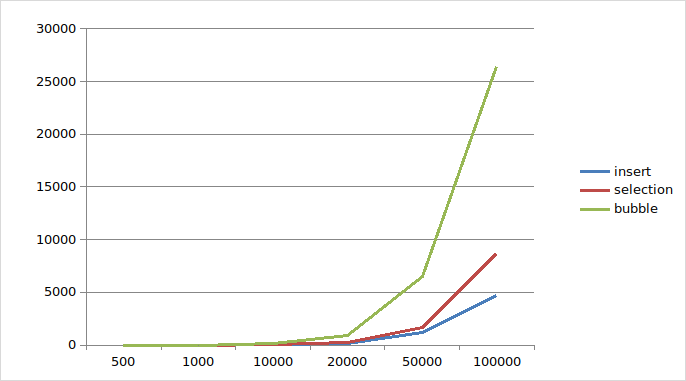
\includegraphics[width=\textwidth]{"../assets/1_1.png"}
    \label{fig:1_1}
\end{figure}


Wykres metod z grupy drugiej:
\begin{figure}[H]
    \centering
    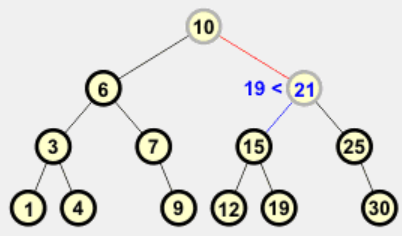
\includegraphics[width=\textwidth]{"../assets/1_2.png"}
    \label{fig:1_2}
\end{figure}

Wspólny wykres
\begin{figure}[H]
    \centering
    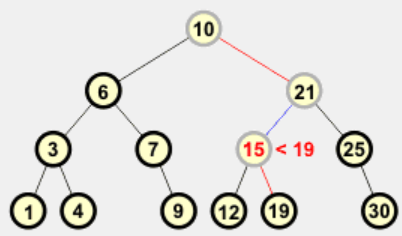
\includegraphics[width=\textwidth]{"../assets/1_3.png"}
    \label{fig:1_3}
\end{figure}
\subsection*{Dla danych posortowanych w kolejności odwrotnej (malejąco)}
Wykres metod z grupy pierwszej:
\begin{figure}[H]
    \centering
    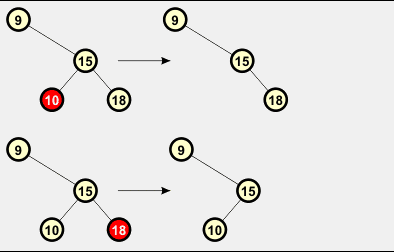
\includegraphics[width=\textwidth]{"../assets/2_1.png"}
    \label{fig:2_1}
\end{figure}


Wykres metod z grupy drugiej:
\begin{figure}[H]
    \centering
    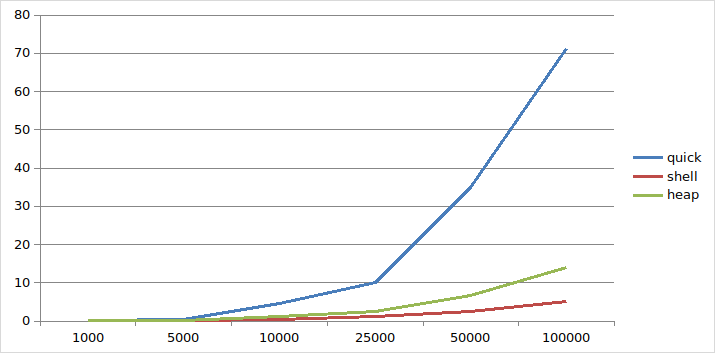
\includegraphics[width=\textwidth]{"../assets/2_2.png"}
    \label{fig:2_2}
\end{figure}

Wspólny wykres
\begin{figure}[H]
    \centering
    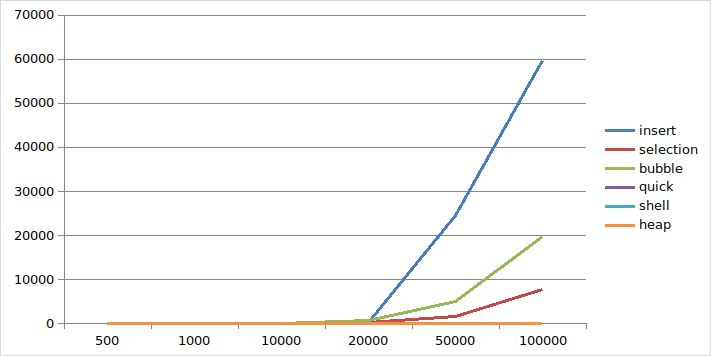
\includegraphics[width=\textwidth]{"../assets/2_3.png"}
    \label{fig:2_3}
\end{figure}
\subsection*{Dla danych posortowanych właściwie (rosnąco)}
Wykres metod z grupy pierwszej:
\begin{figure}[H]
    \centering
    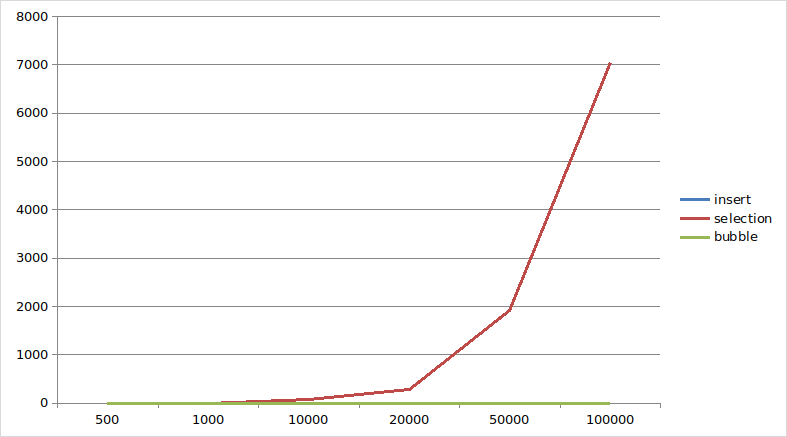
\includegraphics[width=\textwidth]{"../assets/3_1.png"}
    \label{fig:3_1}
\end{figure}


Wykres metod z grupy drugiej:
\begin{figure}[H]
    \centering
    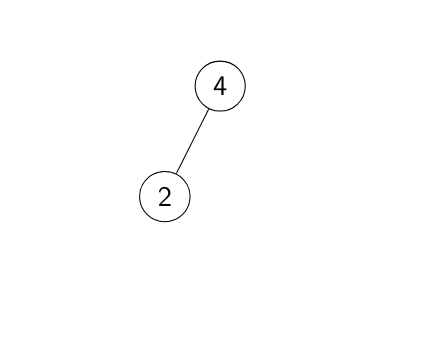
\includegraphics[width=\textwidth]{"../assets/3_2.png"}
    \label{fig:3_2}
\end{figure}

Wspólny wykres
\begin{figure}[H]
    \centering
    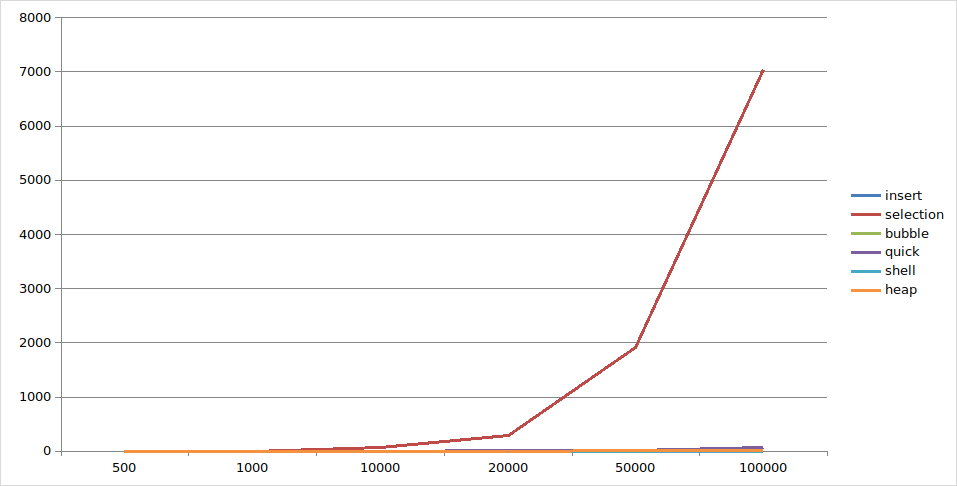
\includegraphics[width=\textwidth]{"../assets/3_3.png"}
    \label{fig:3_3}
\end{figure}


\section*{Podsumowanie}


Algorytmy o złożoności $O(n^2)$ (INSERT, SELECTION, BUBBLE) są wyraźnie nieefektywne dla dużych zbiorów danych, co widać po gwałtownym wzroście czasu wykonania. \newline
Quick Sort i Heap Sort są najbardziej efektywnymi algorytmami w analizie, szczególnie przy dużych zbiorach danych. \newline
Shell Sort oferuje dobrą wydajność i może być preferowanym wyborem w przypadkach, gdzie stabilność czasu wykonania jest istotna, choć nie dorównuje efektywnością Quick Sort i Heap Sort. \newline
Bubble Sort należy unikać w przypadku jakichkolwiek większych zbiorów danych z uwagi na ekstremalnie wysokie czasy wykonania. \newline


\end{document}